\documentclass[journal]{IEEEtran}
\usepackage{graphicx}
\usepackage{booktabs}
\usepackage{hyperref}
% *** CITATION PACKAGES ***
%
\usepackage{cite}
% cite.sty was written by Donald Arseneau
% V1.6 and later of IEEEtran pre-defines the format of the cite.sty package
% \cite{} output to follow that of the IEEE. Loading the cite package will
% result in citation numbers being automatically sorted and properly
% "compressed/ranged". e.g., [1], [9], [2], [7], [5], [6] without using
% cite.sty will become [1], [2], [5]--[7], [9] using cite.sty. cite.sty's
% \cite will automatically add leading space, if needed. Use cite.sty's
% noadjust option (cite.sty V3.8 and later) if you want to turn this off
% such as if a citation ever needs to be enclosed in parenthesis.
% cite.sty is already installed on most LaTeX systems. Be sure and use
% version 5.0 (2009-03-20) and later if using hyperref.sty.
% The latest version can be obtained at:
% http://www.ctan.org/pkg/cite
% The documentation is contained in the cite.sty file itself.

% *** GRAPHICS RELATED PACKAGES ***
%
\ifCLASSINFOpdf
  % \usepackage[pdftex]{graphicx}
  % declare the path(s) where your graphic files are
  % \graphicspath{{../pdf/}{../jpeg/}}
  % and their extensions so you won't have to specify these with
  % every instance of \includegraphics
  % \DeclareGraphicsExtensions{.pdf,.jpeg,.png}
\else
  % or other class option (dvipsone, dvipdf, if not using dvips). graphicx
  % will default to the driver specified in the system graphics.cfg if no
  % driver is specified.
  % \usepackage[dvips]{graphicx}
  % declare the path(s) where your graphic files are
  % \graphicspath{{../eps/}}
  % and their extensions so you won't have to specify these with
  % every instance of \includegraphics
  % \DeclareGraphicsExtensions{.eps}
\fi

\usepackage{amsmath}
% A popular package from the American Mathematical Society that provides
% many useful and powerful commands for dealing with mathematics.
%
% Note that the amsmath package sets \interdisplaylinepenalty to 10000
% thus preventing page breaks from occurring within multiline equations. Use:
%\interdisplaylinepenalty=2500
% after loading amsmath to restore such page breaks as IEEEtran.cls normally
% does. amsmath.sty is already installed on most LaTeX systems. The latest
% version and documentation can be obtained at:
% http://www.ctan.org/pkg/amsmath

% *** SPECIALIZED LIST PACKAGES ***
%
\usepackage{algorithmic}
% algorithmic.sty was written by Peter Williams and Rogerio Brito.
% This package provides an algorithmic environment fo describing algorithms.
% You can use the algorithmic environment in-text or within a figure
% environment to provide for a floating algorithm. Do NOT use the algorithm
% floating environment provided by algorithm.sty (by the same authors) or
% algorithm2e.sty (by Christophe Fiorio) as the IEEE does not use dedicated
% algorithm float types and packages that provide these will not provide
% correct IEEE style captions. The latest version and documentation of
% algorithmic.sty can be obtained at:
% http://www.ctan.org/pkg/algorithms
% Also of interest may be the (relatively newer and more customizable)
% algorithmicx.sty package by Szasz Janos:
% http://www.ctan.org/pkg/algorithmicx

% *** ALIGNMENT PACKAGES ***
%
\usepackage{array}
% Frank Mittelbach's and David Carlisle's array.sty patches and improves
% the standard LaTeX2e array and tabular environments to provide better
% appearance and additional user controls. As the default LaTeX2e table
% generation code is lacking to the point of almost being broken with
% respect to the quality of the end results, all users are strongly
% advised to use an enhanced (at the very least that provided by array.sty)
% set of table tools. array.sty is already installed on most systems. The
% latest version and documentation can be obtained at:
% http://www.ctan.org/pkg/array


% IEEEtran contains the IEEEeqnarray family of commands that can be used to
% generate multiline equations as well as matrices, tables, etc., of high
% quality.

% *** SUBFIGURE PACKAGES ***
\ifCLASSOPTIONcompsoc
  \usepackage[caption=false,font=normalsize,labelfont=sf,textfont=sf]{subfig}
\else
  \usepackage[caption=false,font=footnotesize]{subfig}
\fi
% subfig.sty, written by Steven Douglas Cochran, is the modern replacement
% for subfigure.sty, the latter of which is no longer maintained and is
% incompatible with some LaTeX packages including fixltx2e. However,
% subfig.sty requires and automatically loads Axel Sommerfeldt's caption.sty
% which will override IEEEtran.cls' handling of captions and this will result
% in non-IEEE style figure/table captions. To prevent this problem, be sure
% and invoke subfig.sty's "caption=false" package option (available since
% subfig.sty version 1.3, 2005/06/28) as this is will preserve IEEEtran.cls
% handling of captions.
% Note that the Computer Society format requires a larger sans serif font
% than the serif footnote size font used in traditional IEEE formatting
% and thus the need to invoke different subfig.sty package options depending
% on whether compsoc mode has been enabled.
%
% The latest version and documentation of subfig.sty can be obtained at:
% http://www.ctan.org/pkg/subfig

% *** FLOAT PACKAGES ***
%
%\usepackage{fixltx2e}
% fixltx2e, the successor to the earlier fix2col.sty, was written by
% Frank Mittelbach and David Carlisle. This package corrects a few problems
% in the LaTeX2e kernel, the most notable of which is that in current
% LaTeX2e releases, the ordering of single and double column floats is not
% guaranteed to be preserved. Thus, an unpatched LaTeX2e can allow a
% single column figure to be placed prior to an earlier double column
% figure.
% Be aware that LaTeX2e kernels dated 2015 and later have fixltx2e.sty's
% corrections already built into the system in which case a warning will
% be issued if an attempt is made to load fixltx2e.sty as it is no longer
% needed.
% The latest version and documentation can be found at:
% http://www.ctan.org/pkg/fixltx2e

%\usepackage{stfloats}
% stfloats.sty was written by Sigitas Tolusis. This package gives LaTeX2e
% the ability to do double column floats at the bottom of the page as well
% as the top. (e.g., "\begin{figure*}[!b]" is not normally possible in
% LaTeX2e). It also provides a command:
%\fnbelowfloat
% to enable the placement of footnotes below bottom floats (the standard
% LaTeX2e kernel puts them above bottom floats). This is an invasive package
% which rewrites many portions of the LaTeX2e float routines. It may not work
% with other packages that modify the LaTeX2e float routines. The latest
% version and documentation can be obtained at:
% http://www.ctan.org/pkg/stfloats
% Do not use the stfloats baselinefloat ability as the IEEE does not allow
% \baselineskip to stretch. Authors submitting work to the IEEE should note
% that the IEEE rarely uses double column equations and that authors should try
% to avoid such use. Do not be tempted to use the cuted.sty or midfloat.sty
% packages (also by Sigitas Tolusis) as the IEEE does not format its papers in
% such ways.
% Do not attempt to use stfloats with fixltx2e as they are incompatible.
% Instead, use Morten Hogholm'a dblfloatfix which combines the features
% of both fixltx2e and stfloats:
%
% \usepackage{dblfloatfix}
% The latest version can be found at:
% http://www.ctan.org/pkg/dblfloatfix

% *** PDF, URL AND HYPERLINK PACKAGES ***
%
\usepackage{url}
% url.sty was written by Donald Arseneau. It provides better support for
% handling and breaking URLs. url.sty is already installed on most LaTeX
% systems. The latest version and documentation can be obtained at:
% http://www.ctan.org/pkg/url
% Basically, \url{my_url_here}.

% *** Do not adjust lengths that control margins, column widths, etc. ***
% *** Do not use packages that alter fonts (such as pslatex).         ***
% There should be no need to do such things with IEEEtran.cls V1.6 and later.
% (Unless specifically asked to do so by the journal or conference you plan
% to submit to, of course. )

% correct bad hyphenation here
\hyphenation{op-tical net-works semi-conduc-tor}

\begin{document}
%
% paper title
% Titles are generally capitalized except for words such as a, an, and, as,
% at, but, by, for, in, nor, of, on, or, the, to and up, which are usually
% not capitalized unless they are the first or last word of the title.
% Linebreaks \\ can be used within to get better formatting as desired.
% Do not put math or special symbols in the title.
\title{Worship Analysis}


\author{,~\IEEEmembership{Member,~IEEE,}
        John~Doe,~\IEEEmembership{Fellow,~OSA,}
        and~Jane~Doe,~\IEEEmembership{Life~Fellow,~IEEE}}
%\thanks{M. Shell was with the Department
%of Electrical and Computer Engineering, Georgia Institute of Technology, Atlanta,
%GA, 30332 USA e-mail: (see http://www.michaelshell.org/contact.html).}% <-this % stops a space
%\thanks{J. Doe and J. Doe are with Anonymous University.}% <-this % stops a space
%\thanks{Manuscript received April 19, 2005; revised August 26, 2015.}}

% The paper headers
% \markboth{Journal of \LaTeX\ Class Files,~Vol.~14, No.~8, August~2015}%
% {Shell \MakeLowercase{\textit{et al.}}: Bare Demo of IEEEtran.cls for IEEE Journals}
% The only time the second header will appear is for the odd numbered pages
% after the title page when using the twoside option.
% 
% *** Note that you probably will NOT want to include the author's ***
% *** name in the headers of peer review papers.                   ***
% You can use \ifCLASSOPTIONpeerreview for conditional compilation here if
% you desire.
% conference papers do not typically use \thanks and this command
% is locked out in conference mode. If really needed, such as for
% the acknowledgment of grants, issue a \IEEEoverridecommandlockouts
% after \documentclass

% for over three affiliations, or if they all won't fit within the width
% of the page, use this alternative format:
% 
%\author{\IEEEauthorblockN{Michael Shell\IEEEauthorrefmark{1},
%Homer Simpson\IEEEauthorrefmark{2},
%James Kirk\IEEEauthorrefmark{3}, 
%Montgomery Scott\IEEEauthorrefmark{3} and
%Eldon Tyrell\IEEEauthorrefmark{4}}
%\IEEEauthorblockA{\IEEEauthorrefmark{1}School of Electrical and Computer Engineering\\
%Georgia Institute of Technology,
%Atlanta, Georgia 30332--0250\\ Email: see http://www.michaelshell.org/contact.html}
%\IEEEauthorblockA{\IEEEauthorrefmark{2}Twentieth Century Fox, Springfield, USA\\
%Email: homer@thesimpsons.com}
%\IEEEauthorblockA{\IEEEauthorrefmark{3}Starfleet Academy, San Francisco, California 96678-2391\\
%Telephone: (800) 555--1212, Fax: (888) 555--1212}
%\IEEEauthorblockA{\IEEEauthorrefmark{4}Tyrell Inc., 123 Replicant Street, Los Angeles, California 90210--4321}}




% use for special paper notices
%\IEEEspecialpapernotice{(Invited Paper)}




% make the title area
\maketitle

% As a general rule, do not put math, special symbols or citations
% in the abstract
%\begin{abstract}
%The abstract goes here.
%\end{abstract}

%\begin{IEEEkeywords}
%IEEE, IEEEtran, journal, \LaTeX, paper, template.
% \end{IEEEkeywords}

% For peer review papers, you can put extra information on the cover
% page as needed:
% \ifCLASSOPTIONpeerreview
% \begin{center} \bfseries EDICS Category: 3-BBND \end{center}
% \fi
%
% For peerreview papers, this IEEEtran command inserts a page break and
% creates the second title. It will be ignored for other modes.
\IEEEpeerreviewmaketitle



\section{Introduction}
% no \IEEEPARstart
High-dimensional features has been a hard issue for data scientists in a long period of time. In this work, we evaluated and compared several dimensionality reduction methods, including feature selection, feature projection and feature learning. In order to measure the performance of these methods, we apply it to a 2048-dimension data, and use a SVM classifier to evaluate its performance.

For feature selection methods, we apply forward feature selection, which is rather straightforward, and genetic algorithm, which is harder in comparison. For feature projection methods, we experimented kernel form of principal component analysis(Kernel PCA), linear discriminant analysis(LDA) , auto-encoder(AE) and its variational form(VAE). For feature learning, we analyzed t-distributed stochastic neighborhood embedding(t-SNE) and multi-dimensional scaling(MDS).

The report is organized as follows. In Section~\ref{sec:2}, we introduce the methods we applied in detail; Section~\ref{sec:3} presents our results obtained and analysis of the result. Finally in Section~\ref{sec:4} we conclude this work.

%\hfill mds
 
%\hfill August 26, 2015


\section{Methods}
\label{sec:2}
\subsection{Feature Selection} 
Feature selection is a rather intuitive way to do dimensionality reduction, given its clarity and simplicity. Basic feature selection methods include \textbf{forward and backward feature selecton}, where we either iteratively select or eliminate one feature from the features set until certain criterion is met. A typical advanced feature selection method is \textbf{Genetic Algorithm}, where we simulate the natural process of envolotion to find the optimal subset of features. In this lab work, we experimented with forward feature selection on varience, as well as genetic algorithm to find out the relation between our strategy and its performance.
~\\
\subsubsection{Forward Feature Selection on Variance}
Forward feature selection iteratively select features from the current feature set on some rule until reaches some criterion. In this lab work we choose ``maximum variance'' as the rule, and set the number of features selected as the termination criterion, namely ``top-k variance''. The method is straightforward and simple, with the advantage of requiring less compilation resources and reduced running time.

\subsubsection{Genetic Algorithm}
Genetic algorithm is a bio-inspired optimization algorithm, where the natural rule of envolotion is applied to find the optimal individual in the whole population. After initialization of the whole population of chromosomes, the algorithm performs four steps--fitness evaluation, selection, crossover and selection--iteratively, until the termination criterion is met. We define the chromosomes as a 0-1 mask of all features, where 1 indicates the feature is selected, and 0 indicates not. Following we would describe our implementation of all four steps in this lab work.

For the \textbf{fitness evaluation} part, we design our fitness function as follow:
$$
\mathrm{fitness}(x) = w_s\times S_s + w_f\times S_f
$$
where $S_s, S_f$ are score of the SVM part and features' dimensions part respectively, with $S_s$ defined as the SVM score of the currently selected features, and $S_f$ defined as $\frac{1}{\sum_i x_i}$, which encourages $x$ to have fewer $1$'s, thus selecting fewer dimensions as a result. $w_s$ and $w_f$ is the corresponding weight of these two scores, and could be adjusted to vary each part's contribution to the fitness value.

For \textbf{selection}, we first obtain a probability distribution according to the feature scores, and then sample chromosomes base on that distribution. In detail, we take $p = \frac{\mathrm{fitness}(x_n)}{\sum_n \mathrm{fitness}(x_n)}$, then keep sampling from the current chromosomes base on that until it reaches the previous number of chromosomes. We do this regardless of the possibility that some chromosomes might be sampled more than once, i.e. we allow the new population to consist of identical chromosomes.

\textbf{Crossover} means the process of two chromosomes getting mixed together to produce the next generation, i.e. its siblings. For each chromosome in the current population, we randomly select one other chromosome as its mate, and crossover on a randomly selected cross point. That is, the part in front of this cross point is the same as the former chromosome, and the part behind would belong to the latter one.

Then during \textbf{mutation}, each sibling formed has a certain possibility to mutate, i.e. to have one of its dimension change from $0$ to $1$, or from $1$ to $0$. Note that both mutation and crossover do not happen for granted, but only happen by a certain rate, in order to avoid purely-bad changes that would make the result worse.

An overall process is shown in Figure~\ref{fig:1}. As a feature selection method, it's way more complex than forward/backward feature selection, and could gain better performance as expected. We would show its performance in later sections. 
\begin{figure}[htpb]
  \centering
  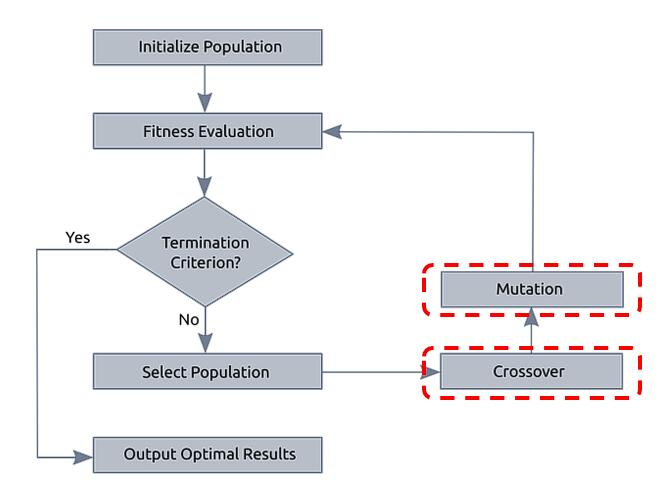
\includegraphics[width=2.5in]{genetic_alg.jpg}
  \caption{process of genetic algorithm}
  \label{fig:1}
  \vspace{-3mm}
\end{figure}

\section{Experiments}
\label{sec:3}
\subsection{Dataset}
The data set we use is \emph{Animals with Attributes (AwA2) dataset} from https://cvml.ist.ac.at/AwA2/. This dataset consists of 37322
images of 50 animal classes with pre-extracted deep learning features for each image. These features has a dimension of 2048.
\subsection{Support Vector Classifier}
In all following experiments, we use support vector classifier (SVC) to classify processed data. The implementation is sklearn.svm.SVC. For the pre-extracted deep-learning features, we use linear kernel and experimented with different hyperparameter $C$'s using k-fold validation, and the result is shown in Table~\ref{tab:1}. We observe that setting $C$ as .. results in the best performance, and we use it as the baseline for following sections. In the following experiments, we sometimes tune $C$ or the kernel to search for optimal results. 
\begin{table}[htbp]
\centering
\caption{Parameters in Genetic Algorithm}
\label{tab:1}
\begin{tabular}{cccc}
\toprule
C&0.1&1&10 \\  % 表格中的内容,用&分开,\\表示下一行
\midrule
Accuracy&0.99&0.99&0.99\\ 
\bottomrule
\end{tabular}
\end{table}
\subsection{Feature Selection}
\subsubsection{Forward Feature Selection}
In this part, we experment with different $k$'s in top-$k$ variance feature selection, while at the same time use $k$-fold validation to find the optimal hyperparameter $C$ in SVM. We experimented with $k=100, 200, \ldots, 1000$, and tested with $C = 0.1, 1, 10$ respectively. The results is shown in Figure~\ref{fig:2}. From the Diagram we can see that the score of the SVMs goes high as $k$ increases. Among three SVMs, that with C = 0.1 performs the best, which is more obvious when the dimensionality is low.
\begin{figure}[htpb]
  \centering
  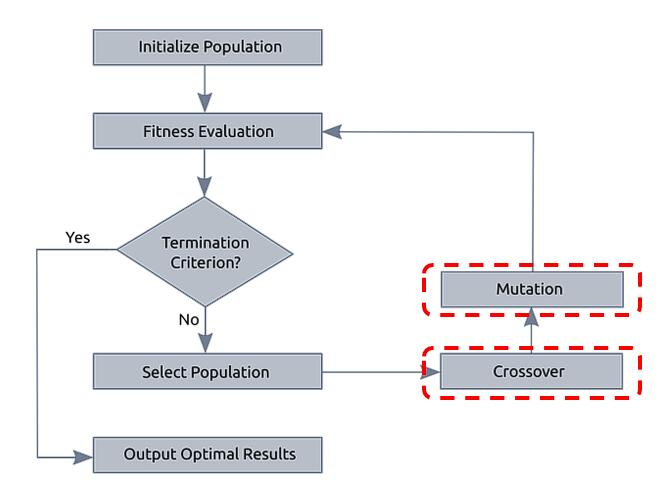
\includegraphics[width=2.5in]{genetic_alg.jpg}
  \caption{Performance of top-k variance}
  \label{fig:2}
  \vspace{-3mm}
\end{figure}

\subsubsection{Genetic Algorithm}
We implement the genetic algorithm with several hyperparameter to be tuned(see Table~\ref{tab:2} for details). Due to the limitation of computation resources, we fix the weight of two scores in our fitness function($w_s$ and $w_f$) to be $0.9$ and $0.1$ respectively, as well as the mutation rate to be $0.5$, and tune the initialization rate(i.e. how many features are selected at first), initialization population, and crossover rate. We also tried different $C$'s when calculating the SVM score $S_s$. The results are shown in Table~\ref{tab:3}. We observe a trend that bigger $IR$ results in higher score, and among different settings, $C=0.1$ seems to perform better than $C=5$. This might due to the fact that once feature dimensions get decreased, data points would become more likely to locate beyond the margin, thus requiring a smaller $C$. We also draw the figure of the highest score in each iteration in Figure~\ref{fig:3}
\begin{table}[htbp]
\centering
\caption{Parameters in Genetic Algorithm}
\label{tab:2}
\begin{tabular}{cc}
\toprule
Parameter&Definition \\  % 表格中的内容,用&分开,\\表示下一行
\midrule
pop&the number of population\\
IR&the rate each feature be selected\\
CR&the rate to perform crossover\\
MR&the rate to perform mutation\\
C&the $C$ for SVC used in fitness computation\\
iter&the number of iterations\\
\bottomrule
\end{tabular}
\end{table}

\begin{table}[htbp]
\centering
\caption{SVM Scores with Regard to Different Settings of Genetic Algorithm}
\label{tab:3}
\begin{tabular}{ccccc}
\toprule

pop&IR&CR&C&iter \\  % 表格中的内容,用&分开,\\表示下一行
\midrule

100&0.1&0.5&1&100 \\

100&0.1&0.5&5&100 \\

100&0.3&0.5&1&100 \\

100&0.3&0.5&5&100 \\
\bottomrule
\end{tabular}
\end{table}
\begin{figure}[htpb]
  \centering
  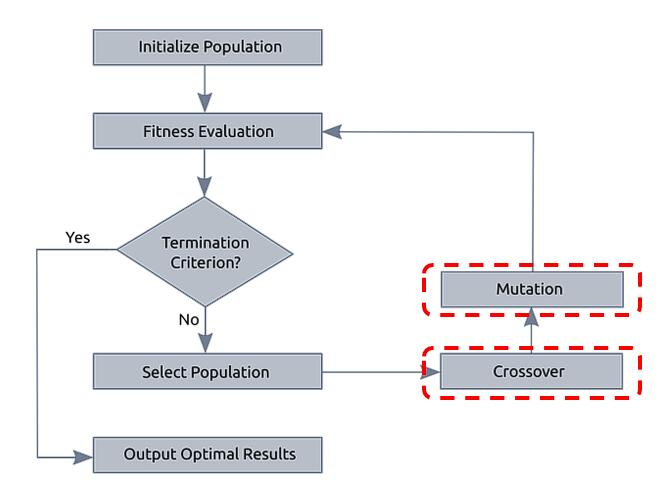
\includegraphics[width=2.5in]{genetic_alg.jpg}
  \caption{Best Score Trend in Genetic Algorithm}
  \label{fig:3}
  \vspace{-3mm}
\end{figure}

\subsubsection{Subsubsection Heading Here}
Subsubsection text here.


% An example of a floating figure using the graphicx package.
% Note that \label must occur AFTER (or within) \caption.
% For figures, \caption should occur after the \includegraphics.
% Note that IEEEtran v1.7 and later has special internal code that
% is designed to preserve the operation of \label within \caption
% even when the captionsoff option is in effect. However, because
% of issues like this, it may be the safest practice to put all your
% \label just after \caption rather than within \caption{}.
%
% Reminder: the "draftcls" or "draftclsnofoot", not "draft", class
% option should be used if it is desired that the figures are to be
% displayed while in draft mode.
%
%\begin{figure}[!t]
%\centering
%\includegraphics[width=2.5in]{myfigure}
% where an .eps filename suffix will be assumed under latex, 
% and a .pdf suffix will be assumed for pdflatex; or what has been declared
% via \DeclareGraphicsExtensions.
%\caption{Simulation results for the network.}
%\label{fig_sim}
%\end{figure}

% Note that the IEEE typically puts floats only at the top, even when this
% results in a large percentage of a column being occupied by floats.


% An example of a double column floating figure using two subfigures.
% (The subfig.sty package must be loaded for this to work.)
% The subfigure \label commands are set within each subfloat command,
% and the \label for the overall figure must come after \caption.
% \hfil is used as a separator to get equal spacing.
% Watch out that the combined width of all the subfigures on a 
% line do not exceed the text width or a line break will occur.
%
%\begin{figure*}[!t]
%\centering
%\subfloat[Case I]{\includegraphics[width=2.5in]{box}%
%\label{fig_first_case}}
%\hfil
%\subfloat[Case II]{\includegraphics[width=2.5in]{box}%
%\label{fig_second_case}}
%\caption{Simulation results for the network.}
%\label{fig_sim}
%\end{figure*}
%
% Note that often IEEE papers with subfigures do not employ subfigure
% captions (using the optional argument to \subfloat[]), but instead will
% reference/describe all of them (a), (b), etc., within the main caption.
% Be aware that for subfig.sty to generate the (a), (b), etc., subfigure
% labels, the optional argument to \subfloat must be present. If a
% subcaption is not desired, just leave its contents blank,
% e.g., \subfloat[].


% An example of a floating table. Note that, for IEEE style tables, the
% \caption command should come BEFORE the table and, given that table
% captions serve much like titles, are usually capitalized except for words
% such as a, an, and, as, at, but, by, for, in, nor, of, on, or, the, to
% and up, which are usually not capitalized unless they are the first or
% last word of the caption. Table text will default to \footnotesize as
% the IEEE normally uses this smaller font for tables.
% The \label must come after \caption as always.
%
%\begin{table}[!t]
%% increase table row spacing, adjust to taste
%\renewcommand{\arraystretch}{1.3}
% if using array.sty, it might be a good idea to tweak the value of
% \extrarowheight as needed to properly center the text within the cells
%\caption{An Example of a Table}
%\label{table_example}
%\centering
%% Some packages, such as MDW tools, offer better commands for making tables
%% than the plain LaTeX2e tabular which is used here.
%\begin{tabular}{|c||c|}
%\hline
%One & Two\\
%\hline
%Three & Four\\
%\hline
%\end{tabular}
%\end{table}


% Note that the IEEE does not put floats in the very first column
% - or typically anywhere on the first page for that matter. Also,
% in-text middle ("here") positioning is typically not used, but it
% is allowed and encouraged for Computer Society conferences (but
% not Computer Society journals). Most IEEE journals/conferences use
% top floats exclusively. 
% Note that, LaTeX2e, unlike IEEE journals/conferences, places
% footnotes above bottom floats. This can be corrected via the
% \fnbelowfloat command of the stfloats package.




\section{Conclusion}
\label{sec:4}
The conclusion goes here.

% conference papers do not normally have an appendix
% if have a single appendix:
%\appendix[Proof of the Zonklar Equations]
% or
%\appendix  % for no appendix heading
% do not use \section anymore after \appendix, only \section*
% is possibly needed

% use appendices with more than one appendix
% then use \section to start each appendix
% you must declare a \section before using any
% \subsection or using \label (\appendices by itself
% starts a section numbered zero.)
%

\appendices
\section{Proof of the First Zonklar Equation}
Appendix one text goes here.

% you can choose not to have a title for an appendix
% if you want by leaving the argument blank
\section{}
Appendix two text goes here.


% use section* for acknowledgment
\section*{Acknowledgment}


The authors would like to thank...





% trigger a \newpage just before the given reference
% number - used to balance the columns on the last page
% adjust value as needed - may need to be readjusted if
% the document is modified later
%\IEEEtriggeratref{8}
% The "triggered" command can be changed if desired:
%\IEEEtriggercmd{\enlargethispage{-5in}}

% references section

% can use a bibliography generated by BibTeX as a .bbl file
% BibTeX documentation can be easily obtained at:
% http://mirror.ctan.org/biblio/bibtex/contrib/doc/
% The IEEEtran BibTeX style support page is at:
% http://www.michaelshell.org/tex/ieeetran/bibtex/
%\bibliographystyle{IEEEtran}
% argument is your BibTeX string definitions and bibliography database(s)
%\bibliography{IEEEabrv,../bib/paper}
%
% <OR> manually copy in the resultant .bbl file
% set second argument of \begin to the number of references
% (used to reserve space for the reference number labels box)
\begin{thebibliography}{1}

\bibitem{IEEEhowto:kopka}
H.~Kopka and P.~W. Daly, \emph{A Guide to \LaTeX}, 3rd~ed.\hskip 1em plus
  0.5em minus 0.4em\relax Harlow, England: Addison-Wesley, 1999.

\end{thebibliography}




% that's all folks
\end{document}


